\documentclass[11pt,a4paper]{article}

% Packages
\usepackage[margin=2.5cm]{geometry}
\usepackage[expansion=false]{microtype}
\usepackage{graphicx}
\usepackage{tikz}
\usetikzlibrary{shapes,arrows.meta,positioning,calc,fit,backgrounds,shadows.blur,decorations.pathmorphing,decorations.pathreplacing}
\usepackage{colortbl}
\usepackage{enumitem}
\usepackage{booktabs}
\usepackage{longtable}
\usepackage{hyperref}
\usepackage{xcolor}
\usepackage{fancyhdr}
\usepackage{titlesec}
\usepackage[most]{tcolorbox}
\usepackage{multicol}
\usepackage{amsmath,amssymb}
\usepackage{multirow}
\usepackage{setspace}
\usepackage{fontawesome5}
\usepackage{listings}

% Spacing
\setlength{\parskip}{3pt plus 1pt minus 1pt}
\setlength{\parindent}{0pt}

% Colors
\definecolor{primary}{HTML}{1A5276}
\definecolor{secondary}{HTML}{2E86C1}
\definecolor{accent}{HTML}{E74C3C}
\definecolor{lightbg}{HTML}{EBF5FB}
\definecolor{defbg}{HTML}{FDF2E9}
\definecolor{greenhl}{HTML}{27AE60}
\definecolor{purplehl}{HTML}{8E44AD}
\definecolor{codebg}{HTML}{F4F6F7}

% Hyperref
\hypersetup{colorlinks=true, linkcolor=primary, urlcolor=secondary, citecolor=primary}

% Code listings style
\lstset{
  backgroundcolor=\color{codebg},
  basicstyle=\ttfamily\small,
  keywordstyle=\color{primary}\bfseries,
  stringstyle=\color{greenhl},
  commentstyle=\color{gray},
  breaklines=true,
  frame=l,
  framerule=2pt,
  rulecolor=\color{secondary!40},
  xleftmargin=8pt,
  framexleftmargin=6pt,
  aboveskip=6pt,
  belowskip=6pt,
  showstringspaces=false,
  language=Python
}

% Header/Footer
\pagestyle{fancy}
\fancyhf{}
\fancyhead[L]{\small\textcolor{primary}{\textbf{E-commerce Development --- Core Concepts}}}
\fancyhead[R]{\small\textcolor{primary}{Lecture Handout}}
\fancyfoot[C]{\small\thepage}
\renewcommand{\headrulewidth}{0.5pt}
\renewcommand{\footrulewidth}{0.3pt}

% Section formatting
\titleformat{\section}{\Large\bfseries\color{primary}}{\thesection}{0.6em}{}[\vspace{2pt}\titlerule]
\titleformat{\subsection}{\large\bfseries\color{secondary}}{\thesubsection}{0.5em}{}
\titleformat{\subsubsection}{\normalsize\bfseries\color{primary}}{\thesubsubsection}{0.5em}{}
\titlespacing*{\section}{0pt}{14pt}{8pt}
\titlespacing*{\subsection}{0pt}{10pt}{5pt}

% Custom boxes
\newtcolorbox{definitionbox}[1][]{
  enhanced, breakable,
  colback=defbg, colframe=orange!60!black,
  colbacktitle=orange!70!black, coltitle=white,
  title={\faIcon{book}~#1}, fonttitle=\bfseries,
  boxrule=0pt, leftrule=4pt, arc=2pt,
  shadow={1mm}{-1mm}{0mm}{black!15},
  top=4pt, bottom=4pt, left=8pt, right=8pt
}
\newtcolorbox{conceptbox}[1][]{
  enhanced, breakable,
  colback=lightbg, colframe=secondary,
  colbacktitle=secondary, coltitle=white,
  title={\faIcon{lightbulb}~#1}, fonttitle=\bfseries,
  boxrule=0pt, leftrule=4pt, arc=2pt,
  shadow={1mm}{-1mm}{0mm}{black!15},
  top=4pt, bottom=4pt, left=8pt, right=8pt
}
\newtcolorbox{alertbox}[1][]{
  enhanced, breakable,
  colback=red!4, colframe=accent,
  colbacktitle=accent, coltitle=white,
  title={\faIcon{exclamation-triangle}~#1}, fonttitle=\bfseries,
  boxrule=0pt, leftrule=4pt, arc=2pt,
  shadow={1mm}{-1mm}{0mm}{black!12},
  top=3pt, bottom=3pt, left=8pt, right=8pt
}
\newtcolorbox{examplebox}[1][]{
  enhanced, breakable,
  colback=green!4, colframe=greenhl,
  colbacktitle=greenhl, coltitle=white,
  title={\faIcon{code}~#1}, fonttitle=\bfseries,
  boxrule=0pt, leftrule=4pt, arc=2pt,
  shadow={1mm}{-1mm}{0mm}{black!12},
  top=3pt, bottom=3pt, left=8pt, right=8pt
}

\begin{document}

% Title
\begin{center}
\vspace*{0.5cm}
{\Huge\bfseries\textcolor{primary}{E-commerce Application}}\\[4pt]
{\Huge\bfseries\textcolor{primary}{Development}}\\[8pt]
{\Huge\bfseries\textcolor{primary}{Core Concepts Handout}}\\[16pt]
{\color{secondary}\rule{0.68\textwidth}{1.5pt}}\\[14pt]
{\Large\textsc{Summer 2026 --- BSIT, 3rd Semester}}\\[8pt]
{\large\textcolor{gray!70!black}{Business Models $\bullet$ Architecture $\bullet$ Payments $\bullet$ Security $\bullet$ CRM/SCM $\bullet$ Marketing $\bullet$ Mobile $\bullet$ Cloud $\bullet$ Ethics}}
\vspace{0.3cm}
\end{center}

\tableofcontents
\newpage

%=============================================================
\section{Introduction to E-commerce}
%=============================================================

\begin{definitionbox}[E-commerce]
Electronic commerce (e-commerce) is the buying, selling, marketing, and servicing of products or services over computer networks such as the Internet, along with the associated data, funds, and document transfers needed to complete each transaction.
\end{definitionbox}

\begin{conceptbox}[Why E-commerce Matters]
E-commerce removes geographic and time barriers between buyers and sellers, letting a business in one city serve customers worldwide, 24 hours a day. For BSIT students, building the applications that power this activity --- storefronts, payment systems, and back-end order processing --- is a core professional skill.
\end{conceptbox}

\subsection{Definition and Scope of E-commerce}
\begin{itemize}[leftmargin=*]
  \item \textbf{E-business vs.\ E-commerce:} E-commerce covers buying/selling transactions; e-business is the broader term covering all digitally-enabled business processes (e-commerce plus internal operations such as HR, manufacturing, and supply chain).
  \item \textbf{Scope:} Includes online retail, digital marketplaces, online banking, e-procurement, online auctions, and digital content/service delivery.
  \item \textbf{Core actors:} Buyers, sellers, intermediaries (marketplaces, payment gateways), and regulators.
\end{itemize}

\subsection{A Brief History and Evolution}
\begin{itemize}[leftmargin=*]
  \item \textbf{1970s--1980s:} Electronic Data Interchange (EDI) allows businesses to exchange documents (invoices, purchase orders) electronically.
  \item \textbf{1994--1995:} The first secure web transactions appear; Amazon and eBay launch, proving consumer e-commerce is viable.
  \item \textbf{Early 2000s:} The dot-com crash filters out weak business models, but survivors (Amazon, Alibaba) scale rapidly.
  \item \textbf{2007--2010s:} Smartphones and app stores give rise to mobile commerce (m-commerce).
  \item \textbf{2010s--present:} Cloud computing, social media, and AI-driven personalization power a global, always-on digital marketplace.
\end{itemize}

\subsection{Traditional Commerce vs.\ E-commerce}
\rowcolors{2}{white}{defbg}
\begin{center}
\begin{tabular}{@{}p{3.0cm}p{5.4cm}p{5.4cm}@{}}
\toprule
\rowcolor{primary!15}
\textbf{Aspect} & \textbf{Traditional Commerce} & \textbf{E-commerce} \\
\midrule
Reach & Local/regional & Global, 24/7 \\
Interaction & Face-to-face & Screen-to-face, self-service \\
Setup Cost & High (physical store, staff) & Lower (hosting, storefront software) \\
Transaction Speed & Slower, manual paperwork & Near-instant, automated \\
Personalization & Limited, generic & Data-driven, highly targeted \\
Payment & Mostly cash/cheque & Cards, e-wallets, EFT, crypto \\
\bottomrule
\end{tabular}
\end{center}

%=============================================================
\section{E-commerce Business Models}
%=============================================================

\begin{definitionbox}[Business Model]
A business model describes who transacts with whom, and how value --- products, services, information, and money --- flows between the parties in an e-commerce system.
\end{definitionbox}

\subsection{Classification by Participants}

\begin{center}
\begin{tikzpicture}[
  ent/.style={rectangle, draw, thick, fill=#1, minimum width=2.8cm, minimum height=1.1cm, align=center, font=\small\bfseries, rounded corners=4pt,
    blur shadow={shadow blur steps=5, shadow xshift=0.5mm, shadow yshift=-0.5mm}},
  arr/.style={{Stealth[length=2.5mm]}-{Stealth[length=2.5mm]}, very thick, primary!60, line width=1.2pt}
]
  \node[ent=blue!12]   (biz) at (0,2.6)     {\faIcon{store}~Business};
  \node[ent=orange!12] (con) at (-3.6,-0.8) {\faIcon{users}~Consumer};
  \node[ent=green!12]  (gov) at (3.6,-0.8)  {\faIcon{university}~Government};

  \draw[arr] (biz) -- node[above left, font=\scriptsize, sloped]{B2C / C2B} (con);
  \draw[arr] (biz) -- node[above right, font=\scriptsize, sloped]{B2G / G2B} (gov);
  \draw[arr] (con) -- node[below, font=\scriptsize]{C2G / G2C} (gov);
\end{tikzpicture}
\end{center}

\begin{itemize}[leftmargin=*]
  \item \textbf{B2B (Business-to-Business):} Manufacturers, wholesalers, and suppliers transacting with each other, e.g., a supplier's e-procurement portal (largest e-commerce segment by transaction value).
  \item \textbf{B2C (Business-to-Consumer):} Businesses selling directly to individual customers, e.g., Amazon, Daraz.
  \item \textbf{C2C (Consumer-to-Consumer):} Individuals trading with each other through an intermediary platform, e.g., eBay, OLX.
  \item \textbf{C2B (Consumer-to-Business):} Individuals offer products/services or set prices for businesses, e.g., freelancing platforms, price-comparison bidding.
  \item \textbf{B2G / G2C:} Businesses and citizens transacting with government agencies, e.g., e-filing taxes, online license renewal.
\end{itemize}

\rowcolors{2}{white}{defbg}
\begin{center}
\begin{tabular}{@{}p{1.6cm}p{4.6cm}p{6.6cm}@{}}
\toprule
\rowcolor{primary!15}
\textbf{Model} & \textbf{Participants} & \textbf{Example} \\
\midrule
B2B & Business $\to$ Business & Steel supplier selling to a car manufacturer online \\
B2C & Business $\to$ Consumer & Amazon, Daraz selling directly to shoppers \\
C2C & Consumer $\to$ Consumer & eBay, OLX classifieds between individuals \\
C2B & Consumer $\to$ Business & Freelancer bidding on a company's project \\
B2G/G2C & Business/Consumer $\leftrightarrow$ Government & Online tax filing, e-procurement tenders \\
\bottomrule
\end{tabular}
\end{center}

\subsection{Revenue Models}
\begin{conceptbox}[Common E-commerce Revenue Models]
\begin{itemize}[leftmargin=*]
  \item \textbf{Merchant/Retail Model:} Selling owned inventory directly to customers at a markup.
  \item \textbf{Marketplace Model:} Hosting third-party sellers and charging a listing or commission fee (e.g., Daraz, Amazon Marketplace).
  \item \textbf{Subscription Model:} Recurring fee for ongoing access to content or services (e.g., streaming, SaaS tools).
  \item \textbf{Freemium Model:} Basic features free, advanced features paid.
  \item \textbf{Advertising Model:} Revenue from displaying ads to a large user base rather than direct sales.
  \item \textbf{Affiliate Model:} Commission earned for referring customers to another merchant's product.
\end{itemize}
\end{conceptbox}

%=============================================================
\section{E-commerce Infrastructure and Web Technologies}
%=============================================================

\begin{definitionbox}[E-commerce Infrastructure]
E-commerce infrastructure is the combination of hardware, software, networks, and standards that allow an online storefront to be built, hosted, and accessed reliably by customers.
\end{definitionbox}

\subsection{The Internet, WWW, and HTTP/HTTPS}
\begin{itemize}[leftmargin=*]
  \item \textbf{Internet:} The global network of interconnected computer networks that carries e-commerce traffic.
  \item \textbf{World Wide Web (WWW):} The system of linked hypertext documents (web pages) accessed via the Internet.
  \item \textbf{HTTP:} The protocol used to request and transfer web pages and data between a browser (client) and a server.
  \item \textbf{HTTPS:} HTTP secured with SSL/TLS encryption --- mandatory for any e-commerce site that handles logins, payments, or personal data.
  \item \textbf{DNS:} Translates human-readable domain names (e.g., \texttt{shop.example.com}) into IP addresses.
\end{itemize}

\begin{conceptbox}[Why HTTPS Is Non-Negotiable for E-commerce]
Without HTTPS, payment details and login credentials travel across the network in plain text and can be intercepted. Browsers actively flag non-HTTPS sites as ``Not Secure,'' which damages customer trust and can violate payment-industry rules (PCI-DSS).
\end{conceptbox}

\subsection{Client-Server Architecture}
\begin{definitionbox}[Client-Server Model]
In the client-server model, a lightweight client (web browser or mobile app) sends requests to a more powerful, centralized server that processes business logic, accesses the database, and returns a response. The server, in turn, queries a database server and returns the result to the client as HTML or JSON.
\end{definitionbox}

\subsection{Front-End vs.\ Back-End Technologies}
\rowcolors{2}{white}{defbg}
\begin{center}
\begin{tabular}{@{}p{2.4cm}p{5.0cm}p{5.2cm}@{}}
\toprule
\rowcolor{primary!15}
\textbf{Layer} & \textbf{Purpose} & \textbf{Example Technologies} \\
\midrule
Front-End & What the customer sees and interacts with in the browser/app & HTML, CSS, JavaScript, React \\
Back-End & Business logic, order processing, authentication & Node.js, PHP, Java, Python (Django/Flask) \\
Database & Persistent storage of products, orders, customers & MySQL, PostgreSQL, MongoDB \\
\bottomrule
\end{tabular}
\end{center}

%=============================================================
\section{Application Architecture for E-commerce Systems}
%=============================================================

\begin{definitionbox}[N-Tier Architecture]
N-tier architecture splits an application into logically separate layers --- typically presentation, application/business logic, and data --- so that each layer can be developed, scaled, and secured independently.
\end{definitionbox}

\subsection{Two-Tier, Three-Tier, and N-Tier Architecture}

\begin{center}
\begin{tikzpicture}[
  tier/.style={rectangle, draw, thick, fill=#1, minimum width=6.0cm, minimum height=1.1cm, align=center, font=\small\bfseries, rounded corners=4pt,
    blur shadow={shadow blur steps=5, shadow xshift=0.5mm, shadow yshift=-0.5mm}},
  arr/.style={{Stealth[length=2.5mm]}-{Stealth[length=2.5mm]}, very thick, primary!60, line width=1.2pt}
]
  \node[tier=blue!12]   (pres) at (0,2.4)  {\faIcon{desktop}~Presentation Tier (UI)};
  \node[tier=orange!12] (app)  at (0,0)    {\faIcon{cogs}~Application Tier (Business Logic)};
  \node[tier=green!12]  (data) at (0,-2.4) {\faIcon{database}~Data Tier (Database)};

  \draw[arr] (pres) -- (app);
  \draw[arr] (app) -- (data);
\end{tikzpicture}
\end{center}

\begin{itemize}[leftmargin=*]
  \item \textbf{Two-Tier:} Client talks directly to the database (thicker client, simple but hard to scale/secure).
  \item \textbf{Three-Tier:} Presentation, business logic, and data are separated --- the standard for modern e-commerce web apps.
  \item \textbf{N-Tier:} Further splits the middle tier (e.g., separate services for catalog, cart, payments) for greater scalability and independent deployment.
\end{itemize}

\subsection{The Model-View-Controller (MVC) Pattern}
\begin{conceptbox}[MVC in E-commerce Applications]
\begin{itemize}[leftmargin=*]
  \item \textbf{Model:} Represents data and business rules, e.g., \texttt{Product}, \texttt{Order}, \texttt{Customer} classes and their database access.
  \item \textbf{View:} Renders the user interface, e.g., the product listing page or the cart page.
  \item \textbf{Controller:} Receives user input (``Add to Cart''), updates the Model, and selects the View to display.
\end{itemize}
MVC keeps UI code, business logic, and data access loosely coupled, so a checkout bug fix does not risk breaking the product catalog page.
\end{conceptbox}

\subsection{Monolithic vs.\ Microservices Architecture}
\rowcolors{2}{white}{defbg}
\begin{center}
\begin{tabular}{@{}p{2.6cm}p{5.2cm}p{5.2cm}@{}}
\toprule
\rowcolor{primary!15}
\textbf{Aspect} & \textbf{Monolithic} & \textbf{Microservices} \\
\midrule
Structure & Single deployable codebase & Independent services (catalog, cart, payments, ...) \\
Scaling & Scale the entire application & Scale only the busy service (e.g., checkout during a sale) \\
Deployment & One deployment for any change & Independent deployment per service \\
Complexity & Simpler initially & More operational complexity (needs orchestration) \\
Best For & Small/early-stage stores & Large-scale platforms (Amazon, Daraz) \\
\bottomrule
\end{tabular}
\end{center}

\subsection{Web Services and API Integration}
\begin{definitionbox}[API]
An Application Programming Interface (API) is a defined contract that lets one software system request data or functionality from another --- e.g., an e-commerce site calling a shipping company's API to get delivery rates.
\end{definitionbox}

\begin{conceptbox}[REST vs.\ SOAP]
\begin{itemize}[leftmargin=*]
  \item \textbf{REST:} Lightweight, uses standard HTTP verbs (GET, POST, PUT, DELETE) and typically JSON; the dominant style for modern e-commerce APIs (payment gateways, shipping, inventory).
  \item \textbf{SOAP:} A stricter, XML-based protocol with built-in standards for security and transactions; still used in some legacy banking/enterprise integrations.
\end{itemize}
\end{conceptbox}

\begin{examplebox}[Illustrative Example: API Call in a Checkout Flow]
When a customer enters their address, the checkout page calls a shipping API: request $\to$ \{origin, destination, weight\} $\to$ response $\to$ \{cost: \$4.50, eta: ``2 days''\}. The storefront never needs to know how the carrier calculates rates --- only the API contract.
\end{examplebox}

%=============================================================
\section{The E-commerce Application Development Lifecycle}
%=============================================================

\begin{definitionbox}[Software Development Lifecycle (SDLC)]
The SDLC is the structured sequence of stages a development team follows to plan, build, test, and maintain an application, ensuring it meets requirements and remains reliable after launch.
\end{definitionbox}

\subsection{Requirements, Design, Development, Testing, Deployment}

\begin{center}
\begin{tikzpicture}[
  step/.style={rectangle, draw, thick, fill=#1, minimum width=2.3cm, minimum height=1.3cm, align=center, font=\footnotesize\bfseries, rounded corners=4pt,
    blur shadow={shadow blur steps=5, shadow xshift=0.5mm, shadow yshift=-0.5mm}},
  arr/.style={-{Stealth[length=2.5mm]}, very thick, primary!60, line width=1.2pt}
]
  \node[step=blue!12]   (s1) at (0,0)    {\faIcon{clipboard-list}\\Requirements};
  \node[step=cyan!12]   (s2) at (2.9,0)  {\faIcon{drafting-compass}\\Design};
  \node[step=orange!12] (s3) at (5.8,0)  {\faIcon{code}\\Development};
  \node[step=yellow!15] (s4) at (0,-2.5)   {\faIcon{vial}\\Testing};
  \node[step=green!12]  (s5) at (2.9,-2.5) {\faIcon{cloud-upload-alt}\\Deployment};
  \node[step=purple!12] (s6) at (5.8,-2.5) {\faIcon{wrench}\\Maintenance};
  \draw[arr] (s1) -- (s2);
  \draw[arr] (s2) -- (s3);
  \draw[arr] (s3.south) to[bend right=18] (s4.north);
  \draw[arr] (s4) -- (s5);
  \draw[arr] (s5) -- (s6);
\end{tikzpicture}
\end{center}

\begin{itemize}[leftmargin=*]
  \item \textbf{Requirements:} Gather business needs --- product catalog size, payment methods, shipping regions, expected traffic.
  \item \textbf{Design:} Define architecture, database schema, UI wireframes, and third-party integrations.
  \item \textbf{Development:} Build front-end, back-end, and database components.
  \item \textbf{Testing:} Functional testing (does checkout work?), security testing, load testing (can it survive a sale?).
  \item \textbf{Deployment:} Release to a live, publicly accessible environment (often cloud-hosted).
  \item \textbf{Maintenance:} Bug fixes, security patches, feature updates, and performance monitoring.
\end{itemize}

\subsection{Key Functional Modules of an E-commerce Application}
\begin{conceptbox}[Core Modules]
\begin{itemize}[leftmargin=*]
  \item \textbf{Product Catalog Module:} Product listings, categories, search, and filtering.
  \item \textbf{User Account Module:} Registration, login, profile, and order history.
  \item \textbf{Shopping Cart Module:} Adding/removing items, quantity updates, price calculation.
  \item \textbf{Checkout and Payment Module:} Address collection, payment processing, order confirmation.
  \item \textbf{Order Management Module:} Order status tracking, invoicing, returns/refunds.
  \item \textbf{Admin/Back-Office Module:} Inventory updates, sales reports, customer support tools.
\end{itemize}
\end{conceptbox}

%=============================================================
\section{Database Design for E-commerce Applications}
%=============================================================

\begin{definitionbox}[E-commerce Database]
The database is the persistent store of all business-critical data --- products, customers, orders, and inventory --- that the application reads and writes on every request.
\end{definitionbox}

\subsection{Core Entities: Products, Customers, Orders, Inventory}
\begin{itemize}[leftmargin=*]
  \item \textbf{Product:} \texttt{product\_id}, name, description, price, category, images.
  \item \textbf{Customer:} \texttt{customer\_id}, name, email, password hash, addresses.
  \item \textbf{Order:} \texttt{order\_id}, \texttt{customer\_id} (foreign key), order date, status, total.
  \item \textbf{Order Item:} \texttt{order\_id}, \texttt{product\_id}, quantity, unit price (links orders to products, many-to-many).
  \item \textbf{Inventory:} \texttt{product\_id}, warehouse location, quantity on hand, reorder threshold.
\end{itemize}

\begin{conceptbox}[How the Tables Relate]
Customer $\to$ Order $\to$ Order Item $\leftarrow$ Product: a customer places many orders (1:N); each order contains many order items (1:N); each order item links back to exactly one product (N:1), so an order item row is what makes products and orders many-to-many.
\end{conceptbox}

\subsection{Entity-Relationship Considerations and Normalization}
\begin{conceptbox}[Why Normalize?]
Normalization removes redundant data (e.g., storing a customer's address once instead of on every order row), preventing update anomalies and saving storage. Most e-commerce schemas target Third Normal Form (3NF), occasionally denormalizing product-listing tables for read speed.
\end{conceptbox}

\subsection{Indexing and Query Performance for Catalogs}
\begin{itemize}[leftmargin=*]
  \item \textbf{Index:} A data structure (commonly a B-tree) that speeds up lookups on a column, e.g., searching products by category or name.
  \item \textbf{Trade-off:} Indexes speed up \texttt{SELECT} queries but slow down \texttt{INSERT}/\texttt{UPDATE}, since the index must also be updated.
  \item \textbf{Caching:} Frequently viewed product pages are often cached (in-memory) so the database is not hit on every request.
\end{itemize}

%=============================================================
\section{Shopping Cart and Checkout Systems}
%=============================================================

\begin{definitionbox}[Shopping Cart]
A shopping cart is a temporary, per-customer record of selected products and quantities, held until the customer completes checkout or abandons the session.
\end{definitionbox}

\subsection{Session and State Management}
\begin{itemize}[leftmargin=*]
  \item \textbf{HTTP is stateless:} Each web request is independent by default, so the server must explicitly track ``whose cart is this?''
  \item \textbf{Session Cookies:} A unique session ID stored in the browser identifies the customer's cart on the server.
  \item \textbf{Persistent Carts:} For logged-in users, cart contents are saved in the database so the cart survives across devices and visits.
  \item \textbf{Guest Carts:} Stored temporarily (cookie or local storage) for customers who have not logged in.
\end{itemize}

\subsection{The Checkout Workflow}
\begin{center}
\begin{tikzpicture}[
  step/.style={rectangle, draw, thick, fill=#1, minimum width=2.4cm, minimum height=1.2cm, align=center, font=\footnotesize\bfseries, rounded corners=4pt,
    blur shadow={shadow blur steps=5, shadow xshift=0.5mm, shadow yshift=-0.5mm}},
  arr/.style={-{Stealth[length=2.5mm]}, very thick, primary!60, line width=1.2pt}
]
  \node[step=blue!12]   (s1) at (0,0)    {\faIcon{search}\\Browse};
  \node[step=cyan!12]   (s2) at (3.0,0)  {\faIcon{shopping-cart}\\Add to\\Cart};
  \node[step=orange!12] (s3) at (6.0,0)  {\faIcon{list-alt}\\Checkout\\Details};
  \node[step=yellow!15] (s4) at (0,-2.6)   {\faIcon{credit-card}\\Payment};
  \node[step=green!12]  (s5) at (3.0,-2.6) {\faIcon{check-circle}\\Order\\Confirmed};
  \node[step=purple!12] (s6) at (6.0,-2.6) {\faIcon{truck}\\Fulfillment};
  \draw[arr] (s1) -- (s2);
  \draw[arr] (s2) -- (s3);
  \draw[arr] (s3.south) to[bend right=18] (s4.north);
  \draw[arr] (s4) -- (s5);
  \draw[arr] (s5) -- (s6);
\end{tikzpicture}
\end{center}

\begin{examplebox}[Illustrative Example: Cart Total Calculation]
Cart contains 2 $\times$ \$15 shirts and 1 $\times$ \$40 jacket, with 5\% sales tax and a flat \$5 shipping fee:
$$
\text{Subtotal} = (2 \times 15) + (1 \times 40) = 70
$$
$$
\text{Tax} = 0.05 \times 70 = 3.5, \qquad \text{Total} = 70 + 3.5 + 5 = 78.5
$$
\end{examplebox}

\subsection{Order Status Lifecycle and Fulfillment}
\begin{conceptbox}[Typical Order States]
\texttt{Placed} $\to$ \texttt{Payment Confirmed} $\to$ \texttt{Processing} $\to$ \texttt{Shipped} $\to$ \texttt{Delivered}, with \texttt{Cancelled} or \texttt{Returned/Refunded} as exception paths. The application must update inventory and notify the customer at each transition.
\end{conceptbox}

%=============================================================
\section{Electronic Payment Systems}
%=============================================================

\begin{definitionbox}[Electronic Payment System]
An electronic payment system is the set of technologies and institutions that transfer funds from a customer to a merchant digitally, without physical cash changing hands.
\end{definitionbox}

\subsection{Types of E-Payment Instruments}
\rowcolors{2}{white}{defbg}
\begin{center}
\begin{tabular}{@{}p{2.6cm}p{5.0cm}p{5.2cm}@{}}
\toprule
\rowcolor{primary!15}
\textbf{Instrument} & \textbf{Description} & \textbf{Example} \\
\midrule
Credit/Debit Card & Bank-issued card charged/debited immediately or with a bill cycle & Visa, Mastercard \\
E-Wallet & Stored-value or linked account accessed via app & PayPal, Easypaisa, JazzCash \\
Electronic Funds Transfer (EFT) & Direct bank-to-bank transfer & Online/mobile banking transfer \\
Buy Now, Pay Later (BNPL) & Installment financing at checkout & Point-of-sale installment plans \\
Cryptocurrency & Decentralized digital currency & Bitcoin, Ethereum payments \\
Cash on Delivery (COD) & Cash paid at the time of delivery & Common in emerging e-commerce markets \\
\bottomrule
\end{tabular}
\end{center}

\subsection{Payment Gateway Architecture and Transaction Flow}
\begin{definitionbox}[Payment Gateway]
A payment gateway is a service that securely captures, encrypts, and routes a customer's payment details from the merchant's checkout page to the banking network for authorization.
\end{definitionbox}

\begin{center}
\begin{tikzpicture}[
  step/.style={rectangle, draw, thick, fill=#1, minimum width=2.3cm, minimum height=1.3cm, align=center, font=\footnotesize\bfseries, rounded corners=4pt,
    blur shadow={shadow blur steps=5, shadow xshift=0.5mm, shadow yshift=-0.5mm}},
  arr/.style={-{Stealth[length=2.5mm]}, very thick, primary!60, line width=1.2pt}
]
  \node[step=blue!12]   (cu) at (0,0)    {\faIcon{user}\\Customer};
  \node[step=cyan!12]   (me) at (3.1,0)  {\faIcon{store}\\Merchant\\Checkout};
  \node[step=orange!12] (gw) at (6.2,0)  {\faIcon{lock}\\Payment\\Gateway};
  \node[step=yellow!15] (ac) at (9.3,0)  {\faIcon{university}\\Acquiring\\Bank};
  \node[step=green!12]  (cn) at (9.3,-2.4)  {\faIcon{network-wired}\\Card\\Network};
  \node[step=purple!12] (is) at (6.2,-2.4)  {\faIcon{university}\\Issuing\\Bank};
  \draw[arr] (cu) -- (me);
  \draw[arr] (me) -- (gw);
  \draw[arr] (gw) -- (ac);
  \draw[arr] (ac) -- (cn);
  \draw[arr] (cn) -- (is);
  \draw[arr] (is.west) to[bend right=15] node[below, font=\scriptsize]{Approve/Decline} (me.south);
\end{tikzpicture}
\end{center}

\begin{conceptbox}[Reading the Flow]
The customer's card details never touch the merchant's own servers directly in a well-designed system --- the gateway tokenizes them. The issuing bank (customer's bank) checks funds/fraud and returns an approval or decline, which travels back through the same chain in milliseconds.
\end{conceptbox}

\subsection{PCI-DSS and Compliance Basics}
\begin{definitionbox}[PCI-DSS]
The Payment Card Industry Data Security Standard (PCI-DSS) is a set of security requirements that any business storing, processing, or transmitting cardholder data must follow, e.g., never storing the card verification code (CVV) after authorization.
\end{definitionbox}
\begin{itemize}[leftmargin=*]
  \item Use a certified payment gateway so raw card numbers never touch your own database.
  \item Encrypt cardholder data in transit (TLS) and at rest.
  \item Restrict access to payment data on a need-to-know basis and log all access.
  \item Regularly test systems for vulnerabilities (scans, penetration testing).
\end{itemize}

%=============================================================
\section{E-commerce Security}
%=============================================================

\begin{definitionbox}[E-commerce Security]
E-commerce security is the set of practices and technologies that protect a storefront's data, transactions, and customers from unauthorized access, alteration, or disruption.
\end{definitionbox}

\subsection{Security Goals}
\begin{conceptbox}[The Core Security Goals]
\begin{itemize}[leftmargin=*]
  \item \textbf{Confidentiality:} Only authorized parties can read sensitive data (customer details, payment info).
  \item \textbf{Integrity:} Data cannot be altered undetected in transit or storage (e.g., an order total cannot be silently changed).
  \item \textbf{Availability:} The store stays online and responsive, even under attack (e.g., resisting a Denial-of-Service attack).
  \item \textbf{Authentication:} Verifying that a user or system really is who it claims to be (login, API keys).
  \item \textbf{Non-repudiation:} A party cannot later deny having made a transaction (e.g., digitally signed order confirmations).
\end{itemize}
\end{conceptbox}

\subsection{Encryption and SSL/TLS}
\begin{center}
\begin{tikzpicture}[
  lyr/.style={rectangle, draw, thick, fill=#1, minimum width=6.4cm, minimum height=1.0cm, align=center, font=\small\bfseries, rounded corners=4pt,
    blur shadow={shadow blur steps=5, shadow xshift=0.5mm, shadow yshift=-0.5mm}},
  arr/.style={-{Stealth[length=2.5mm]}, very thick, primary!60, line width=1.2pt}
]
  \node[lyr=blue!12]   (app) at (0,3.6)  {\faIcon{shopping-cart}~Application Layer (checkout logic)};
  \node[lyr=cyan!12]   (auth) at (0,2.2) {\faIcon{key}~Authentication \& Session Security};
  \node[lyr=orange!12] (tls) at (0,0.8)  {\faIcon{lock}~SSL/TLS Encryption in Transit};
  \node[lyr=yellow!15] (fw) at (0,-0.6)  {\faIcon{shield-alt}~Firewall / Web Application Firewall};
  \node[lyr=green!12]  (net) at (0,-2.0) {\faIcon{network-wired}~Network Layer};
  \draw[arr] (app) -- (auth);
  \draw[arr] (auth) -- (tls);
  \draw[arr] (tls) -- (fw);
  \draw[arr] (fw) -- (net);
\end{tikzpicture}
\end{center}

\begin{itemize}[leftmargin=*]
  \item \textbf{Symmetric Encryption:} Same key encrypts and decrypts (fast; used for bulk data once a connection is established).
  \item \textbf{Asymmetric Encryption:} A public/private key pair; the public key encrypts, only the matching private key decrypts (used to establish the SSL/TLS session).
  \item \textbf{SSL/TLS Handshake:} Browser and server exchange certificates and negotiate a shared session key before any data (including passwords or card numbers) is transmitted.
  \item \textbf{Digital Certificate:} Issued by a trusted Certificate Authority (CA) to prove a website's identity to the browser.
\end{itemize}

\subsection{Common Web Threats}
\rowcolors{2}{white}{defbg}
\begin{center}
\begin{tabular}{@{}p{2.6cm}p{5.2cm}p{5.2cm}@{}}
\toprule
\rowcolor{primary!15}
\textbf{Threat} & \textbf{How It Works} & \textbf{Mitigation} \\
\midrule
SQL Injection & Malicious SQL inserted through an input field to manipulate the database & Parameterized queries, input validation \\
Cross-Site Scripting (XSS) & Malicious script injected into a page and run in another user's browser & Output encoding, Content Security Policy \\
Cross-Site Request Forgery (CSRF) & Tricks a logged-in user's browser into submitting an unwanted request & CSRF tokens, same-site cookies \\
Man-in-the-Middle (MITM) & Attacker intercepts traffic between client and server & Enforce HTTPS/TLS everywhere \\
Phishing & Fake site/email tricks users into revealing credentials & User education, email authentication (SPF/DKIM) \\
\bottomrule
\end{tabular}
\end{center}

\subsection{Digital Signatures and Certificates}
\begin{definitionbox}[Digital Signature]
A digital signature uses the sender's private key to sign data (e.g., an order confirmation or software update), letting anyone verify --- with the sender's public key --- that the data is authentic and unaltered.
\end{definitionbox}
\begin{examplebox}[Illustrative Example: Verifying a Signed Receipt]
A merchant signs a receipt with its private key. The customer's app checks the signature using the merchant's public certificate; if the check succeeds, the receipt is provably from that merchant and has not been tampered with.
\end{examplebox}

%=============================================================
\section{Customer Relationship Management and Supply Chain Management}
%=============================================================

\begin{definitionbox}[Customer Relationship Management (CRM)]
CRM is the set of practices, strategies, and software an organization uses to manage interactions with current and potential customers throughout the customer lifecycle.
\end{definitionbox}

\subsection{CRM Concepts and the Customer Lifecycle}
\begin{itemize}[leftmargin=*]
  \item \textbf{Acquisition:} Attracting new visitors and converting them into first-time buyers.
  \item \textbf{Retention:} Encouraging repeat purchases through loyalty programs, personalized offers, and good service.
  \item \textbf{Win-back:} Re-engaging customers who have stopped purchasing (e.g., ``we miss you'' discount emails).
  \item \textbf{360-Degree View:} Combining browsing history, purchase history, and support tickets into one customer profile.
\end{itemize}

\subsection{Recommendation Engines and Personalization}
\begin{conceptbox}[How Recommendation Engines Work]
\begin{itemize}[leftmargin=*]
  \item \textbf{Collaborative Filtering:} ``Customers who bought this also bought...'' --- based on the behavior of similar users.
  \item \textbf{Content-Based Filtering:} Recommends items similar in attributes (category, brand) to what the customer already viewed or bought.
  \item \textbf{Personalization:} Tailoring homepage banners, search ranking, and email offers to an individual customer's behavior.
\end{itemize}
\end{conceptbox}

\subsection{Supply Chain and Inventory Management Integration}
\begin{definitionbox}[Supply Chain Management (SCM)]
SCM coordinates the flow of goods from suppliers through manufacturing/warehousing to the final customer, ensuring the right product is in the right place when an order is placed.
\end{definitionbox}
\begin{itemize}[leftmargin=*]
  \item \textbf{Real-time Inventory Sync:} The storefront must reflect true stock levels to avoid selling out-of-stock items.
  \item \textbf{Warehouse Management System (WMS):} Tracks stock location, picking, and packing for fulfillment.
  \item \textbf{Drop-shipping:} The store forwards the order to a supplier who ships directly to the customer, so the retailer never holds inventory.
  \item \textbf{Just-in-Time (JIT):} Ordering stock only as needed to minimize holding costs.
\end{itemize}

%=============================================================
\section{Digital Marketing for E-commerce}
%=============================================================

\begin{definitionbox}[Digital Marketing]
Digital marketing is the use of online channels --- search engines, social media, email, and advertising networks --- to attract, convert, and retain e-commerce customers.
\end{definitionbox}

\subsection{Search Engine Optimization (SEO) and Search Engine Marketing (SEM)}
\rowcolors{2}{white}{defbg}
\begin{center}
\begin{tabular}{@{}p{2.6cm}p{5.2cm}p{5.2cm}@{}}
\toprule
\rowcolor{primary!15}
\textbf{Aspect} & \textbf{SEO (Organic)} & \textbf{SEM (Paid)} \\
\midrule
Cost & Free traffic, but takes time & Pay-per-click, immediate visibility \\
Method & Keywords, quality content, backlinks, page speed & Paid search ads (e.g., Google Ads) \\
Longevity & Long-term, compounding benefit & Stops when the budget stops \\
\bottomrule
\end{tabular}
\end{center}

\subsection{Email, Social Media, and Affiliate Marketing}
\begin{itemize}[leftmargin=*]
  \item \textbf{Email Marketing:} Cart-abandonment reminders, promotional newsletters, order confirmations.
  \item \textbf{Social Media Marketing:} Organic posts and paid ads on platforms like Instagram and Facebook, often linking directly to product pages (social commerce).
  \item \textbf{Affiliate Marketing:} Independent partners earn a commission for traffic/sales they refer, tracked via unique links.
  \item \textbf{Influencer Marketing:} Paying content creators to showcase products to their audience.
\end{itemize}

\subsection{The Marketing/Conversion Funnel}
\begin{conceptbox}[Funnel Stages, Widest to Narrowest]
Awareness $\to$ Interest $\to$ Consideration $\to$ Conversion $\to$ Retention --- each stage narrows as fewer visitors advance, forming the classic ``funnel'' shape.
\end{conceptbox}

\begin{itemize}[leftmargin=*]
  \item \textbf{Awareness:} Customer discovers the brand via ads, SEO, or social media.
  \item \textbf{Interest:} Customer browses the catalog or reads reviews/content.
  \item \textbf{Consideration:} Customer compares products/prices, may add to cart.
  \item \textbf{Conversion:} Customer completes checkout and pays.
  \item \textbf{Retention:} Post-purchase engagement (emails, loyalty programs) drives repeat orders.
\end{itemize}

%=============================================================
\section{Mobile Commerce (M-Commerce)}
%=============================================================

\begin{definitionbox}[Mobile Commerce (M-Commerce)]
M-commerce is e-commerce conducted through mobile devices --- smartphones and tablets --- using either a mobile browser or a dedicated app.
\end{definitionbox}

\subsection{Mobile Web vs.\ Native Apps}
\rowcolors{2}{white}{defbg}
\begin{center}
\begin{tabular}{@{}p{2.6cm}p{5.2cm}p{5.2cm}@{}}
\toprule
\rowcolor{primary!15}
\textbf{Aspect} & \textbf{Mobile Web} & \textbf{Native App} \\
\midrule
Access & Any browser, no install & Must be downloaded/installed \\
Development Cost & One codebase for all devices & Often separate iOS/Android codebases \\
Performance & Depends on network/browser & Faster, works offline for cached content \\
Features & Limited device access & Full access (camera, push notifications, GPS) \\
Discoverability & Found via search engines & Found via app stores \\
\bottomrule
\end{tabular}
\end{center}

\subsection{Responsive Design and Progressive Web Apps}
\begin{conceptbox}[Responsive Design]
Responsive web design uses flexible layouts (CSS media queries, fluid grids) so the same storefront renders well on a phone, tablet, and desktop --- essential since most e-commerce traffic today is mobile.
\end{conceptbox}
\begin{definitionbox}[Progressive Web App (PWA)]
A PWA is a website built to behave like a native app --- installable, works offline via a service worker cache, and can send push notifications --- without requiring an app-store download.
\end{definitionbox}

%=============================================================
\section{Cloud Computing and Scalability for E-commerce}
%=============================================================

\begin{definitionbox}[Cloud Computing]
Cloud computing delivers computing resources --- servers, storage, databases --- over the Internet on demand, letting an e-commerce business pay only for what it uses instead of owning physical hardware.
\end{definitionbox}

\subsection{IaaS, PaaS, and SaaS for Hosting}
\rowcolors{2}{white}{defbg}
\begin{center}
\begin{tabular}{@{}p{2.6cm}p{5.4cm}p{5.0cm}@{}}
\toprule
\rowcolor{primary!15}
\textbf{Model} & \textbf{What the Provider Manages} & \textbf{Example} \\
\midrule
IaaS & Servers, storage, networking --- you manage the OS and app & Virtual machines, cloud storage \\
PaaS & Runtime, OS, and infrastructure --- you manage only the app code & Managed app-hosting platforms \\
SaaS & The entire application, ready to use & Hosted storefront builders \\
\bottomrule
\end{tabular}
\end{center}

\subsection{Load Balancing, Caching, and Auto-Scaling}
\begin{center}
\begin{tikzpicture}[
  node1/.style={rectangle, draw, thick, fill=#1, minimum width=2.6cm, minimum height=1.0cm, align=center, font=\small\bfseries, rounded corners=4pt,
    blur shadow={shadow blur steps=5, shadow xshift=0.5mm, shadow yshift=-0.5mm}},
  arr/.style={-{Stealth[length=2.5mm]}, very thick, primary!60, line width=1.2pt}
]
  \node[node1=blue!12]   (lb)  at (3.3,2.2)   {\faIcon{random}~Load Balancer};
  \node[node1=orange!12] (w1)  at (0,0)       {\faIcon{server}~Web Server 1};
  \node[node1=orange!12] (w2)  at (3.3,0)     {\faIcon{server}~Web Server 2};
  \node[node1=orange!12] (w3)  at (6.6,0)     {\faIcon{server}~Web Server $N$};
  \node[node1=green!12]  (ca)  at (0,-2.2)    {\faIcon{bolt}~Cache};
  \node[node1=purple!12] (db)  at (6.6,-2.2)  {\faIcon{database}~Database};

  \draw[arr] (lb) -- (w1);
  \draw[arr] (lb) -- (w2);
  \draw[arr] (lb) -- (w3);
  \draw[arr] (w1) -- (ca);
  \draw[arr] (w3) -- (db);
\end{tikzpicture}
\end{center}

\begin{itemize}[leftmargin=*]
  \item \textbf{Load Balancer:} Distributes incoming traffic across multiple identical web servers so no single server is overwhelmed.
  \item \textbf{Caching:} Stores frequently requested data (product pages, session data) in fast memory to reduce database load.
  \item \textbf{Auto-Scaling:} Automatically adds or removes server instances based on real-time traffic (e.g., during a flash sale).
\end{itemize}

\subsection{High Availability and Disaster Recovery Basics}
\begin{conceptbox}[Staying Online]
\begin{itemize}[leftmargin=*]
  \item \textbf{Redundancy:} Multiple servers/data centers so a single failure does not take the store offline.
  \item \textbf{Backups:} Regular database backups so data can be restored after corruption or attack.
  \item \textbf{Failover:} Automatic switch to a standby system if the primary system fails.
\end{itemize}
\end{conceptbox}

%=============================================================
\section{Legal, Ethical, and Tax Issues in E-commerce}
%=============================================================

\begin{definitionbox}[Cyberlaw]
Cyberlaw is the body of legal rules governing online transactions, digital contracts, data protection, and electronic evidence.
\end{definitionbox}

\begin{alertbox}[Key Concerns]
\begin{itemize}[leftmargin=*]
  \item \textbf{Data Privacy:} Collecting, storing, and processing customer data responsibly (e.g., GDPR-style consent and data-minimization principles).
  \item \textbf{Consumer Protection:} Clear return/refund policies, accurate product descriptions, and protection against fraud.
  \item \textbf{Digital Contracts and E-Signatures:} An online ``I agree'' click or e-signature can be legally binding, provided identity and intent are verifiable.
  \item \textbf{Intellectual Property:} Protecting trademarks, product images, and content from unauthorized copying; respecting others' IP in listings.
  \item \textbf{Digital Taxation:} Sales tax/VAT collection rules differ by jurisdiction and are often tied to the buyer's location, not just the seller's.
  \item \textbf{Cross-Border Trade:} Customs duties, import regulations, and currency conversion complicate international orders.
\end{itemize}
\end{alertbox}

\begin{conceptbox}[Building Ethical E-commerce Systems]
\begin{itemize}[leftmargin=*]
  \item Be transparent about pricing, shipping costs, and how customer data is used.
  \item Avoid dark patterns (e.g., hidden fees revealed only at the last checkout step, fake urgency countdowns).
  \item Secure customer data proportionally to its sensitivity, and disclose breaches promptly.
  \item Ensure accessibility (e.g., screen-reader compatibility) so the store is usable by customers with disabilities.
\end{itemize}
\end{conceptbox}

%=============================================================
\section{Emerging Trends in E-commerce}
%=============================================================

\begin{definitionbox}[Why Trends Matter]
E-commerce technology evolves quickly; staying current with emerging trends helps developers design applications that remain competitive and meet rising customer expectations.
\end{definitionbox}

\subsection{AI, Chatbots, and Conversational Commerce}
\begin{itemize}[leftmargin=*]
  \item \textbf{AI-Powered Personalization:} Dynamic pricing, personalized search ranking, and product recommendations.
  \item \textbf{Chatbots:} Automated, always-available customer support and guided shopping assistants.
  \item \textbf{Conversational Commerce:} Completing a purchase directly within a chat app or voice assistant.
  \item \textbf{Visual Search:} Customers search using a photo instead of text keywords.
\end{itemize}

\subsection{Social Commerce, Voice Commerce, and Blockchain}
\begin{conceptbox}[New Shopping Channels]
\begin{itemize}[leftmargin=*]
  \item \textbf{Social Commerce:} Buying directly within social media apps (e.g., Instagram/Facebook shops) without leaving the platform.
  \item \textbf{Voice Commerce:} Ordering through voice assistants (e.g., ``reorder my usual coffee'').
  \item \textbf{Blockchain in E-commerce:} Used for transparent supply-chain tracking, smart contracts, and cryptocurrency payments.
  \item \textbf{Augmented Reality (AR):} ``Try before you buy'' experiences, e.g., virtually placing furniture in a room.
\end{itemize}
\end{conceptbox}

%=============================================================
\section{Core Quantitative Foundations for E-commerce}
%=============================================================

\begin{definitionbox}[Why Quantitative Literacy Matters]
Every major decision in e-commerce --- pricing, marketing spend, inventory levels --- is guided by a small set of standard business metrics and calculations that a developer or analyst must be able to compute and interpret.
\end{definitionbox}

\subsection{Key Performance Indicators (KPIs)}
\rowcolors{2}{white}{defbg}
\begin{center}
\begin{tabular}{@{}p{3.4cm}p{9.8cm}@{}}
\toprule
\rowcolor{primary!15}
\textbf{KPI} & \textbf{Formula / Meaning} \\
\midrule
Conversion Rate & $\dfrac{\text{Orders}}{\text{Visitors}} \times 100\%$ --- share of visitors who purchase \\
\addlinespace
Average Order Value (AOV) & $\dfrac{\text{Total Revenue}}{\text{Number of Orders}}$ --- average amount spent per order \\
\addlinespace
Customer Lifetime Value (CLV) & Avg.\ Order Value $\times$ Purchase Frequency $\times$ Customer Lifespan \\
\addlinespace
Cart Abandonment Rate & $\dfrac{\text{Carts Created} - \text{Orders Completed}}{\text{Carts Created}} \times 100\%$ \\
\addlinespace
Bounce Rate & Share of visitors who leave after viewing only one page \\
\addlinespace
Return on Ad Spend (ROAS) & $\dfrac{\text{Revenue from Ads}}{\text{Ad Spend}}$ \\
\bottomrule
\end{tabular}
\end{center}

\subsection{Pricing, Discount, and Tax Calculations}
\begin{conceptbox}[Order Total Formula]
$$
\text{Order Total} = (\text{Subtotal} - \text{Discount}) \times (1 + \text{Tax Rate}) + \text{Shipping}
$$
Discounts are usually applied \emph{before} tax; shipping is usually added \emph{after} tax, though policies vary by jurisdiction and platform.
\end{conceptbox}

\subsection{Break-Even and ROI Basics}
\begin{definitionbox}[Break-Even Point]
The break-even point is the number of units that must be sold so that total revenue exactly equals total cost (fixed costs plus variable costs), leaving zero profit or loss.
\end{definitionbox}
$$
\text{Break-Even Units} = \frac{\text{Fixed Costs}}{\text{Price per Unit} - \text{Variable Cost per Unit}}
$$
\begin{definitionbox}[Return on Investment (ROI)]
$$
\text{ROI} = \frac{\text{Net Profit}}{\text{Cost of Investment}} \times 100\%
$$
\end{definitionbox}

%=============================================================
\section{Exam-Oriented Worked Examples}
%=============================================================

\begin{examplebox}[Worked Example 1: Conversion Rate]
An online store receives 8,000 visitors in a month and completes 240 orders:
$$
\text{Conversion Rate} = \frac{240}{8000} \times 100\% = 3\%
$$
\end{examplebox}

\begin{examplebox}[Worked Example 2: Average Order Value (AOV)]
In one week, a store generates \$12,500 in revenue from 250 orders:
$$
AOV = \frac{12500}{250} = \$50
$$
\end{examplebox}

\begin{examplebox}[Worked Example 3: Customer Lifetime Value (CLV)]
A customer places an average order of \$50, orders 4 times per year, and remains a customer for 3 years:
$$
CLV = 50 \times 4 \times 3 = \$600
$$
\end{examplebox}

\begin{examplebox}[Worked Example 4: Cart Abandonment Rate]
In a month, 1,000 carts are created but only 350 result in completed orders:
$$
\text{Abandonment Rate} = \frac{1000 - 350}{1000} \times 100\% = 65\%
$$
\end{examplebox}

\begin{examplebox}[Worked Example 5: Discount and Sales Tax on an Order]
An order subtotal is \$200, a 10\% discount coupon is applied, and sales tax is 5\%, with a flat \$6 shipping fee:
$$
\text{After Discount} = 200 \times (1 - 0.10) = 180
$$
$$
\text{Total} = 180 \times (1 + 0.05) + 6 = 189 + 6 = \$195
$$
\end{examplebox}

\begin{examplebox}[Worked Example 6: Payment Gateway Transaction Fee]
A payment gateway charges 2.9\% + \$0.30 per transaction on a \$50 order:
$$
\text{Fee} = (0.029 \times 50) + 0.30 = 1.45 + 0.30 = \$1.75
$$
$$
\text{Merchant Receives} = 50 - 1.75 = \$48.25
$$
\end{examplebox}

\begin{examplebox}[Worked Example 7: Return on Ad Spend (ROAS)]
A \$500 ad campaign generates \$2,750 in attributed revenue:
$$
ROAS = \frac{2750}{500} = 5.5
$$
Every \$1 spent on ads returned \$5.50 in revenue.
\end{examplebox}

\begin{examplebox}[Worked Example 8: Break-Even Units for an Online Store]
Fixed monthly costs (hosting, salaries) are \$4,000; each unit sells for \$25 with a variable cost of \$15:
$$
\text{Break-Even Units} = \frac{4000}{25 - 15} = \frac{4000}{10} = 400 \text{ units}
$$
\end{examplebox}

%=============================================================
\section{Quick Revision Glossary}
%=============================================================

\rowcolors{2}{white}{defbg}
\begin{longtable}{@{}p{3.3cm}p{10.2cm}@{}}
\toprule
\rowcolor{primary!15}
\textbf{Term} & \textbf{One-Line Meaning} \\
\midrule
\endhead
E-commerce & Buying, selling, and servicing products/services over computer networks. \\
\addlinespace
EDI & Electronic Data Interchange; structured business-document exchange between computers. \\
\addlinespace
B2B & Business-to-Business transactions, e.g., supplier to manufacturer. \\
\addlinespace
B2C & Business-to-Consumer transactions, e.g., store to shopper. \\
\addlinespace
C2C & Consumer-to-Consumer transactions via an intermediary platform. \\
\addlinespace
C2B & Consumer-to-Business transactions, e.g., freelance bidding. \\
\addlinespace
Affiliate Marketing & Paying partners a commission for referred traffic or sales. \\
\addlinespace
Client-Server Architecture & Clients send requests; a central server processes logic and data. \\
\addlinespace
Three-Tier Architecture & Presentation, application logic, and data layers are separated. \\
\addlinespace
MVC Pattern & Splits an app into Model (data), View (UI), and Controller (input handling). \\
\addlinespace
Monolithic Architecture & Entire application deployed as a single unit. \\
\addlinespace
Microservices & Application split into independently deployable services. \\
\addlinespace
API & A defined contract letting one system request data/functions from another. \\
\addlinespace
REST & Lightweight API style using HTTP verbs and typically JSON. \\
\addlinespace
Shopping Cart & Temporary record of a customer's selected items before checkout. \\
\addlinespace
Checkout & The workflow of collecting address, payment, and confirming an order. \\
\addlinespace
Payment Gateway & Service that securely captures and routes payment details for authorization. \\
\addlinespace
E-Wallet & App or account holding stored value for digital payments. \\
\addlinespace
EFT & Electronic Funds Transfer; direct bank-to-bank money movement. \\
\addlinespace
BNPL & Buy Now, Pay Later; installment financing offered at checkout. \\
\addlinespace
Cash on Delivery (COD) & Payment made in cash when the order is delivered. \\
\addlinespace
PCI-DSS & Payment Card Industry Data Security Standard for handling card data. \\
\addlinespace
SSL/TLS & Protocols that encrypt data in transit between browser and server. \\
\addlinespace
SQL Injection & Attack that inserts malicious SQL through an input field. \\
\addlinespace
Cross-Site Scripting (XSS) & Attack that injects malicious scripts into pages viewed by other users. \\
\addlinespace
CSRF & Cross-Site Request Forgery; tricks a logged-in browser into an unwanted request. \\
\addlinespace
Digital Signature & Private-key-based proof that data is authentic and unaltered. \\
\addlinespace
CRM & Customer Relationship Management; managing the customer lifecycle. \\
\addlinespace
SCM & Supply Chain Management; coordinating goods from supplier to customer. \\
\addlinespace
SEO & Search Engine Optimization; improving organic search visibility. \\
\addlinespace
SEM & Search Engine Marketing; paid search advertising. \\
\addlinespace
M-Commerce & E-commerce conducted via mobile devices. \\
\addlinespace
Progressive Web App (PWA) & Website that behaves like an installable, offline-capable app. \\
\addlinespace
Cloud Computing & On-demand delivery of computing resources over the Internet. \\
\addlinespace
IaaS / PaaS / SaaS & Infrastructure- / Platform- / Software-as-a-Service cloud models. \\
\addlinespace
Load Balancer & Distributes incoming traffic across multiple servers. \\
\addlinespace
Conversion Rate & Percentage of visitors who complete a purchase. \\
\addlinespace
Average Order Value (AOV) & Average amount spent per completed order. \\
\addlinespace
Customer Lifetime Value (CLV) & Total revenue expected from a customer over the relationship. \\
\addlinespace
Cart Abandonment Rate & Share of created carts that do not result in a completed order. \\
\addlinespace
ROAS & Return on Ad Spend; revenue generated per dollar of advertising. \\
\addlinespace
Break-Even Point & Sales volume at which total revenue equals total cost. \\
\bottomrule
\end{longtable}

%=============================================================
\section{Question Bank Blueprint (80 Marks Support)}
%=============================================================

\begin{conceptbox}[Suggested 80 Marks Distribution]
\begin{itemize}[leftmargin=*]
  \item \textbf{Section A:} MCQs and definitions (20 marks)
  \item \textbf{Section B:} Short conceptual questions (20 marks)
  \item \textbf{Section C:} Descriptive/theory questions (20 marks)
  \item \textbf{Section D:} Numerical/problem-solving questions (20 marks)
\end{itemize}
\end{conceptbox}

\subsection{Important Theory Questions}
\begin{itemize}[leftmargin=*]
  \item Differentiate e-commerce and e-business with examples.
  \item Explain the B2B, B2C, C2C, and C2B business models with real-world examples.
  \item Compare traditional commerce with e-commerce across at least four dimensions.
  \item Explain three-tier architecture and why it is preferred over two-tier for e-commerce apps.
  \item Differentiate monolithic and microservices architecture, with a suitable use case for each.
  \item Explain the Model-View-Controller (MVC) pattern in the context of an e-commerce application.
  \item Describe the complete software development lifecycle for an e-commerce application.
  \item Explain the role of session management in maintaining a shopping cart.
  \item Describe the end-to-end transaction flow through a payment gateway.
  \item Explain PCI-DSS and why it matters for any business accepting card payments.
  \item Differentiate SQL Injection, XSS, and CSRF, and describe one mitigation for each.
  \item Explain the difference between CRM and SCM, and how they support an e-commerce business.
  \item Differentiate SEO and SEM as digital marketing strategies.
  \item Explain the advantages and disadvantages of native apps versus mobile web for m-commerce.
  \item Explain IaaS, PaaS, and SaaS, and how cloud computing supports e-commerce scalability.
  \item Discuss legal, ethical, and tax issues relevant to running an online store.
  \item Describe two emerging trends transforming e-commerce today.
\end{itemize}

\subsection{Important Numerical/Analytical Questions}
\begin{itemize}[leftmargin=*]
  \item Compute the conversion rate given visitor and order counts.
  \item Compute the Average Order Value (AOV) given total revenue and number of orders.
  \item Compute Customer Lifetime Value (CLV) given average order value, purchase frequency, and customer lifespan.
  \item Compute the cart abandonment rate given carts created and orders completed.
  \item Compute an order's final total given a subtotal, a percentage discount, a tax rate, and a shipping fee.
  \item Compute the payment gateway fee and net amount received by a merchant for a given transaction.
  \item Compute the Return on Ad Spend (ROAS) given ad spend and attributed revenue.
  \item Compute the break-even number of units given fixed costs, price per unit, and variable cost per unit.
\end{itemize}

\subsection{Sample MCQs with Answer Key}
\begin{enumerate}[leftmargin=*]
  \item Which business model describes a freelancer bidding on a company's project?\\
  (a) B2B \quad (b) B2C \quad (c) C2B \quad (d) C2C
  \item Which architecture layer is responsible for storing product and order data?\\
  (a) Presentation Tier \quad (b) Application Tier \quad (c) Data Tier \quad (d) Client Tier
  \item Which design pattern separates an application into Model, View, and Controller?\\
  (a) MVC \quad (b) MVP \quad (c) SOA \quad (d) ETL
  \item Which protocol encrypts data in transit between a browser and a web server?\\
  (a) HTTP \quad (b) FTP \quad (c) SSL/TLS \quad (d) SMTP
  \item Which attack inserts malicious SQL through an unvalidated input field?\\
  (a) XSS \quad (b) CSRF \quad (c) SQL Injection \quad (d) Phishing
  \item Which standard governs the secure handling of cardholder data?\\
  (a) GDPR \quad (b) PCI-DSS \quad (c) ISO 9001 \quad (d) HIPAA
  \item Which metric divides total revenue by the number of completed orders?\\
  (a) Conversion Rate \quad (b) Average Order Value \quad (c) ROAS \quad (d) Bounce Rate
  \item Which cloud service model requires the customer to manage only their application code?\\
  (a) IaaS \quad (b) PaaS \quad (c) SaaS \quad (d) On-premises
  \item Which component distributes incoming traffic across multiple web servers?\\
  (a) Firewall \quad (b) Load Balancer \quad (c) Database \quad (d) Payment Gateway
\end{enumerate}
\begin{conceptbox}[Answer Key]
1--(c), 2--(c), 3--(a), 4--(c), 5--(c), 6--(b), 7--(b), 8--(b), 9--(b)
\end{conceptbox}

%=============================================================
\section{Summary}
%=============================================================

\begin{examplebox}[Key Takeaways]
\begin{itemize}[leftmargin=*]
  \item E-commerce spans B2B, B2C, C2C, C2B, and government-linked models, each with distinct revenue strategies.
  \item Modern e-commerce applications rely on client-server, three-tier/N-tier, and increasingly microservices architectures, built through a standard SDLC.
  \item Well-designed databases, session-managed shopping carts, and secure payment gateways form the technical backbone of any storefront.
  \item Security (encryption, PCI-DSS, defenses against SQL Injection/XSS/CSRF) and legal/ethical compliance are non-negotiable for customer trust.
  \item CRM, SCM, and digital marketing (SEO, SEM, the conversion funnel) drive customer acquisition and retention.
  \item Mobile commerce, cloud scalability, and emerging trends (AI, social/voice commerce, blockchain) are reshaping how storefronts are built and accessed.
  \item KPIs such as conversion rate, AOV, CLV, cart abandonment, and ROAS give developers and managers a shared, quantitative language for measuring success.
\end{itemize}
\end{examplebox}

\end{document}
